%%%%%%%%%%%%%%%%%%%%%%% file template.tex %%%%%%%%%%%%%%%%%%%%%%%%%
%
% This is a general template file for the LaTeX package SVJour3
% for Springer journals.          Springer Heidelberg 2010/09/16
%
% Copy it to a new file with a new name and use it as the basis
% for your article. Delete % signs as needed.
%
% This template includes a few options for different layouts and
% content for various journals. Please consult a previous issue of
% your journal as needed.
%
%%%%%%%%%%%%%%%%%%%%%%%%%%%%%%%%%%%%%%%%%%%%%%%%%%%%%%%%%%%%%%%%%%%
%
% First comes an example EPS file -- just ignore it and
% proceed on the \documentclass line
% your LaTeX will extract the file if required
\begin{filecontents*}{example.eps}
%!PS-Adobe-3.0 EPSF-3.0
%%BoundingBox: 19 19 221 221
%%CreationDate: Mon Sep 29 1997
%%Creator: programmed by hand (JK)
%%EndComments
gsave
newpath
  20 20 moveto
  20 220 lineto
  220 220 lineto
  220 20 lineto
closepath
2 setlinewidth
gsave
  .4 setgray fill
grestore
stroke
grestore
\end{filecontents*}
%
\RequirePackage{fix-cm}
%
%\documentclass{svjour3}                     % onecolumn (standard format)
%\documentclass[smallcondensed]{svjour3}     % onecolumn (ditto)
\documentclass[smallextended]{svjour3}       % onecolumn (second format)
%\documentclass[twocolumn]{svjour3}          % twocolumn
%
\smartqed  % flush right qed marks, e.g. at end of proof
%
\usepackage{graphicx}
\usepackage[numbers]{natbib}%TODO delete before submission
\usepackage{amsmath}
%
% \usepackage{mathptmx}      % use Times fonts if available on your TeX system
%
% insert here the call for the packages your document requires
%\usepackage{latexsym}
% etc.
%
% please place your own definitions here and don't use \def but
% \newcommand{}{}
%
% Insert the name of "your journal" with
% \journalname{myjournal}
%
\begin{document}

\title{The Furuta Pendulum
%\thanks{Grants or other notes
%about the article that should go on the front page should be
%placed here. General acknowledgments should be placed at the end of the article.}
}
\subtitle{Technical Report}

%\titlerunning{Short form of title}        % if too long for running head

\author{Maximilian Gehrke \and Tabea Wilke \and Yannik Frisch %etc.
}

%\authorrunning{Short form of author list} % if too long for running head

\institute{F. Author \at
              first address \\
              Tel.: +123-45-678910\\
              Fax: +123-45-678910\\
              \email{fauthor@example.com}           %  \\
%             \emph{Present address:} of F. Author  %  if needed
           \and
           S. Author \at
              second address
}

\date{Received: date / Accepted: date}
% The correct dates will be entered by the editor


\maketitle

\begin{abstract}
The Furuta Pendulum is an example of a complex non-linear system and therefore 
of big interest in control system theory. It consists of one controllable arm 
rotating in the horizontal plane and one pendulum uncontrollably moving in the 
vertical plane, which is attached to the end of this arm.\\
The non-linearities result from an interplay between gravitational, Coriolis and centripetal forces. \\
XX We present an overview over it's technical details and proposed algorithms to solve the control problem. XX
\keywords{First keyword \and Second keyword \and More}
% \PACS{PACS code1 \and PACS code2 \and more}
% \subclass{MSC code1 \and MSC code2 \and more}
\end{abstract}
\section{Introduction}
Many examples of the field of control engineering like aircraft landing, 
aircraft stabilizing and many more can be very well modelled by an inverted 
pendulum \cite{akhtaruzzaman2010modeling}. As a reaction to problems with the 
limited movement of the cart from 
the inverted pendulum, the furuta pendulum (also called rotary inverted 
pendulum) 
has been developed by 
\citeauthor{furuta1992swing}. The advantages of the furuta pendulum are that it 
needs less space and one moving arm is directly linked to the motor, therefore, 
the dynamics is less unmodeled thanks to a power transmission mechanism 
\cite{furuta1992swing}. The furuta pendulum is an underactuated problem, this 
means that there two degrees of freedom ($\phi,\ \theta$), 
but only one arm is directly controlled by the motor. This is the one which 
changes the angle $\phi$ in the horizontal plane. The other arm called pendulum 
is attached to 
the end of the controlled arm and therefore is moved indirectly by it in the 
vertical plane with angle $\theta$ 
\cite{spong1998underactuated,tedrake2009underactuated}. The whole system is 
highly non-linear as a result of an interplay between gravitational, coriolis 
and centripetal forces.
\begin{figure}[h]
	\centering
	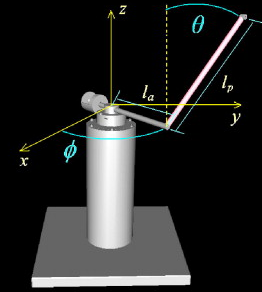
\includegraphics[width=0.5\linewidth]{pendulum}
	\caption{The furuta pendulum, figure from \cite{la2009new}}
	\label{fig:pendulum}
\end{figure}
Finally, there are two different types of control problems. First, bringing the 
flexible arm from a hanging position to a position which is nearly upright, 
further called "swing-up". Second, if the arm is nearly upright with low enough 
speed, balancing it to hold this state stable, called "stabilization". 
\subsection{Definitions}
The system consists of an arm with length $l_r$ mounted to a DC motor, which is 
able to apply a torque of $\tau$ to it. It has a mass of $m_r$ which is 
located at $l_1$ alongside the arm. Another arm with length $l_p$ and mass 
$m_p$ %located at $\frac{l_p}{2}$ 
is attached to the remaining side of the 
first arm. Both arms have a moment of inertia $J_r$ and $J_p$ respectively. The 
counter force to the input torque is the viscous damping $B_r$ because of the 
bearings of the motor. As the pendulum is not controlled directly, the only 
force it is applied to is damping at the connection to the arm $B_p$. The angle 
$\theta$ is zero if the pendulum is in an perfectly upright position.
The only influence we can take on the system is the voltage $V_m$ we give to 
the DC motor.
\section{Mathematical Modelling 
\cite{furuta1992swing,gafvert2016modelling,ozbek2010swing,zhang2011optimal}}
For later derivation of the Lagrangian, the kinetic and potential engergies of 
the furuta pendulum are needed. Therefore, the kinematics of the pendulums 
center of gravity can be described by 
\[\begin{cases}
x&=l_r\cos\phi-l_{p}\sin\theta\sin\phi \\ 
y&=l_r\sin\phi+l_{p}\sin\theta\cos\phi \\ 
z&=l_{p}\cos\theta
\end{cases} \] 
The relative velocity of the pendulum to the arm can be represented by 
\[ \begin{cases}
\dot{x}&=-l_a\ \sin \phi \dot{\phi}-l_{p}\ \cos\phi \sin\theta\dot{\phi}-l_{p} 
\ \sin\phi \cos\theta\dot{\theta} \\ 
\dot{y} &=l_a\ \cos\phi\dot{\phi}-l_{p} \ \sin\phi \sin\theta\dot{\phi}+l_{p} 
\ \cos\theta \cos\phi\dot{\theta} \\
 \dot{z}&=-l_{p} \ \sin\theta\dot{\theta}
\end{cases}\]
For the energy terms a squared velocity is needed, which is the scalar product 
of the squared velocities in all directions:
\begin{align*}v^2&=\dot{x}^2+\dot{y}^2+\dot{z}^2\\
&=(l_a^2+l_p^2\ 
\sin^2\theta)\dot{\phi}^2+l_p^2\dot{\theta}^2+2l_al_p\dot{\phi}\dot{\theta}\cos 
\theta\end{align*} %TODO ich kann die Herleitung dafür in den Anhang packen, 
%falls 
%gewünscht
First of all, we will derive the equations of motion through the Euler-Lagrange 
method. The Lagrangian function can be obtained by the difference of the 
kinetic and potential energies $L=T-V$, with $T$ as the total sum of the 
kinetic energies in the system and $V$ the total potential energies. Lagrange's 
Equation follows \[ 
\frac{d}{dt}\left(\frac{\partial L}{\partial 
\dot{q_i}}\right)-\frac{\partial 
L}{\partial 
q_i}=0 \] Thereby, the variables $q_i$ are called generalized coordinates. For 
the furuta pendulum this is $\dot{q}(t)^T = \left[\frac{\partial 
\phi(t)}{\partial t} \frac{\partial \theta(t)}{\partial t} \right]$ which leads 
to 
\begin{align*}
	\frac{\partial^2 L}{\partial t\partial \dot{\phi}}-\frac{\partial 
	L}{\partial \phi}&=\tau - B_r\dot{\phi}\\
	\frac{\partial^2 L}{\partial t\partial \dot{\theta}}-\frac{\partial 
	L}{\partial \theta}&=-B_p\dot{\theta}
\end{align*}
The only potential energy which is in the system is the one of the pendulum:
\[V_{total}=V_{pendulum}=m_pgz= m_pgl_{p}\cos\theta\]
\bibliographystyle{spbasic}      % basic style, author-year citations
\bibliography{furuta.bib}   % name your BibTeX data base




\end{document}
% end of file template.tex

